\documentclass[12pt]{article}
\usepackage{amssymb,amsmath}% http://ctan.org/pkg/{amssymb,amsmath}
\usepackage{braket}% http://ctan.org/pkg/braket
\usepackage[margin=0.1in]{geometry}
\usepackage{graphicx}
\usepackage{subcaption}
\usepackage{amsmath}
\usepackage{relsize}
\usepackage{pdflscape}
\begin{document}




\[\text{\bf{The Data Generating Process (DGP):}}\]
\[\text{Customer $C$ Spend on Order $X$} = t*c*r*d + \epsilon \]
\[t = \text{Whether or not the customer recieved the experimental treatment } t \in [1,1.01].\]
\[c = \text{Customer's mean order amount in dollars where } c \sim \mathcal{N}(\$100,\$25).\]
\[r = \text{Scalar corresponding to mean retailer order amount where } r \sim \mathcal{N}(1.0,0.05).\]
\[d = \text{Scalar corresponding to mean order amount for that day of the week where } d \in [0.7,1.3].\]
\[\epsilon = \text{Random noise where } \epsilon \sim \mathcal{N}(\$25,\$1).\]
\[\text{Let the number of orders $N$ placed by Customer $C$ } \sim exp(\lambda = 1).\]

\[\text{\bf{The Model:}}\]
\[ y = \beta_0 + \beta_1X_1 + \beta_2X_2 + \beta_3X_3 + \beta_4X_4 \]
\[\text{...where $X_1$ is the treatment, $X_2$ is the customer's mean order amount prior to treatment,}\] 
\[\text{$X_3$ is the retailer's mean order amount prior to treatment,}\] 
\[\text{and $X_4$ is the mean order amount for that day of the week prior to treatment.}\]

\newpage
\begin{landscape}
\begin{center}
\Large{Required Sample Size Estimates Taken Via Interpolation}
\end{center}
\begin{table}[h]
\begin{tabular}{c|ccccccccc}
                                                                              & \textbf{\begin{tabular}[c]{@{}c@{}}Method \\ I\end{tabular}} & \textbf{\begin{tabular}[c]{@{}c@{}}Method \\ II\end{tabular}} & \textbf{\begin{tabular}[c]{@{}c@{}}Method\\ III\end{tabular}} & \textbf{\begin{tabular}[c]{@{}c@{}}Method \\ IV\end{tabular}} & \textbf{\begin{tabular}[c]{@{}c@{}}Method \\ V\end{tabular}} & \textbf{\begin{tabular}[c]{@{}c@{}}Method \\ VI\end{tabular}} & \textbf{\begin{tabular}[c]{@{}c@{}}Method \\ VII\end{tabular}} & \textbf{\begin{tabular}[c]{@{}c@{}}Method \\ VIII\end{tabular}} & \textbf{\begin{tabular}[c]{@{}c@{}}Method \\ IX\end{tabular}} \\ \hline
\textbf{\begin{tabular}[c]{@{}c@{}}Points Used\end{tabular}} 
& 3  &5    &7 & 3  &5    &7 & 3  &5    &7                                            \\ \hline                                                                              
\textbf{\begin{tabular}[c]{@{}c@{}}Simulations Per Point\end{tabular}} 
& 100    & 100  & 100    & 200 & 200  & 200  & 300 & 300  & 300   
\\ \hline                                                                              
\textbf{\begin{tabular}[c]{@{}c@{}} Total Simulations \\ Required\end{tabular}} 
& 300 & 500 & 700 & 600 & 1,000 & 1,400 & 900 & 1,500 & 2,100                                        \\ \hline
\textbf{\begin{tabular}[c]{@{}c@{}}Mean Difference \\ in Estimated Power (Std.)\end{tabular}} &
\begin{tabular}[c]{@{}c@{}}0.04   \\ (0.104) \end{tabular} &          
\begin{tabular}[c]{@{}c@{}}0.034  \\ (0.034)\end{tabular} &       
\begin{tabular}[c]{@{}c@{}}-0.008 \\ (0.047)\end{tabular} &  
\begin{tabular}[c]{@{}c@{}}0.039  \\ (0.089)\end{tabular} &    
\begin{tabular}[c]{@{}c@{}}0.025  \\ (0.024)\end{tabular} &  
\begin{tabular}[c]{@{}c@{}}-0.022 \\ (0.041)\end{tabular} &
\begin{tabular}[c]{@{}c@{}}0.046  \\ (0.061)\end{tabular} &
\begin{tabular}[c]{@{}c@{}}0.025  \\ (0.022)\end{tabular} &
\begin{tabular}[c]{@{}c@{}}-0.021 \\ (0.033)\end{tabular} 
\\ \hline                                                                              
\textbf{\begin{tabular}[c]{@{}c@{}}Mean Estimated \\ Sample Size (Std.)\end{tabular}}    & 
\begin{tabular}[c]{@{}c@{}}25,147 \\ (5,208)\end{tabular} &          
\begin{tabular}[c]{@{}c@{}}23,497 \\ (1,836)\end{tabular} &       
\begin{tabular}[c]{@{}c@{}}21,101 \\ (2,434)\end{tabular} &  
\begin{tabular}[c]{@{}c@{}}24,752 \\ (4,698)\end{tabular} &    
\begin{tabular}[c]{@{}c@{}}22,883 \\ (1,237)\end{tabular} &  
\begin{tabular}[c]{@{}c@{}}20,244 \\ (2,036)\end{tabular} &
\begin{tabular}[c]{@{}c@{}}24,925 \\ (3,690)\end{tabular} &
\begin{tabular}[c]{@{}c@{}}22,956 \\ (1,054)\end{tabular} &
\begin{tabular}[c]{@{}c@{}}20,231 \\ (1,491)\end{tabular}
\\ \hline                                                                              
\textbf{\begin{tabular}[c]{@{}c@{}}Mean Estimation Time \\ in Minutes (Std.)\end{tabular}}    & 
\begin{tabular}[c]{@{}c@{}}0.761 \\ (0.625)\end{tabular} &          
\begin{tabular}[c]{@{}c@{}}0.474 \\ (0.1)\end{tabular} &       
\begin{tabular}[c]{@{}c@{}}0.659 \\ (0.081)\end{tabular} &  
\begin{tabular}[c]{@{}c@{}}1.447 \\ (1.116)\end{tabular} &    
\begin{tabular}[c]{@{}c@{}}1.239 \\ (0.28)\end{tabular} &  
\begin{tabular}[c]{@{}c@{}}1.464 \\ (0.295)\end{tabular} &
\begin{tabular}[c]{@{}c@{}}1.879 \\ (1.409)\end{tabular} &
\begin{tabular}[c]{@{}c@{}}1.411 \\ (0.196)\end{tabular} &
\begin{tabular}[c]{@{}c@{}}1.976 \\ (0.198)\end{tabular}  
\\ \hline                                                                              
\textbf{\begin{tabular}[c]{@{}c@{}} Verification Simulations \end{tabular}}
& 500  & 500  & 500  & 500  & 500  & 500   & 500    & 500  & 500                                          
\end{tabular}
\end{table}
\begin{center}
Simulations were conducted on dual Intel Xeon CPU E5-2670 processors.
\end{center}
\end{landscape}

\newpage

\noindent
\begin{figure}[b]
\centering
\begin{subfigure}{.32\textwidth}
    \centering
    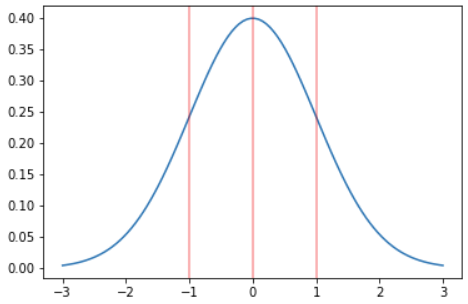
\includegraphics[width=0.75\textwidth]{sd_3.png}
    \caption[short]{$\mu$ +/- [1]$\sigma$ \\with 500 iterations.}
    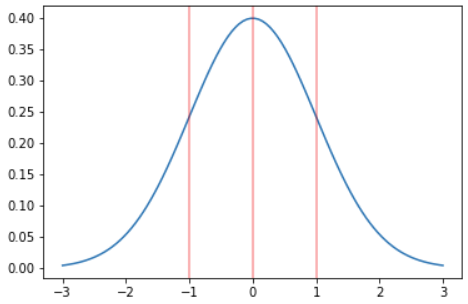
\includegraphics[width=0.75\textwidth]{sd_3.png}
    \caption[short]{$\mu$ +/- [1,2]$\sigma$ \\with 500 iterations.}
    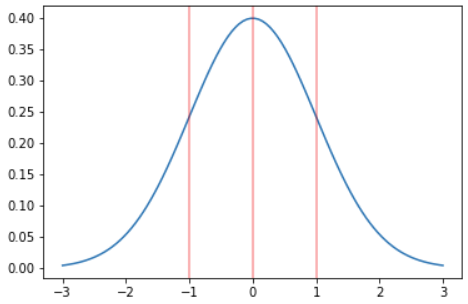
\includegraphics[width=0.75\textwidth]{sd_3.png}
    \caption[short]{$\mu$ +/- [1,2,3]$\sigma$ \\with 500 iterations.}
\end{subfigure}
\begin{subfigure}{.32\textwidth}
    \centering
    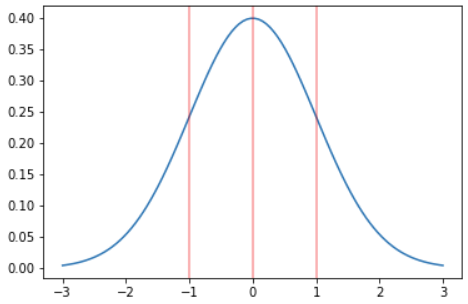
\includegraphics[width=0.75\textwidth]{sd_3.png}
    \caption[short]{$\mu$ +/- [1]$\sigma$ \\with 1,000 iterations.}
    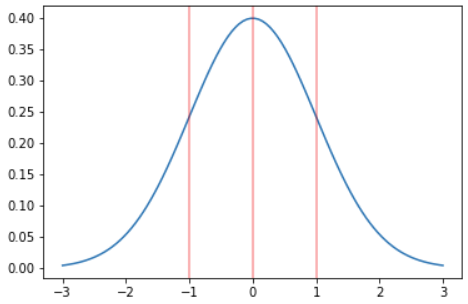
\includegraphics[width=0.75\textwidth]{sd_3.png}
    \caption[short]{$\mu$ +/- [1,2]$\sigma$ \\with 1,000 iterations.}
    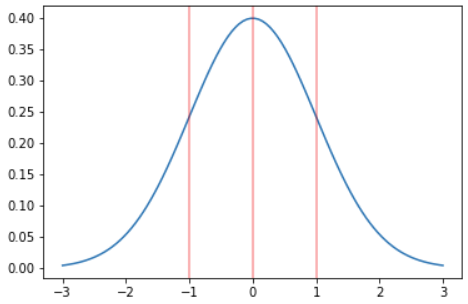
\includegraphics[width=0.75\textwidth]{sd_3.png}
    \caption[short]{$\mu$ +/- [1,2,3]$\sigma$ \\with 1,000 iterations.}
\end{subfigure}
\begin{subfigure}{.32\textwidth}
    \centering
    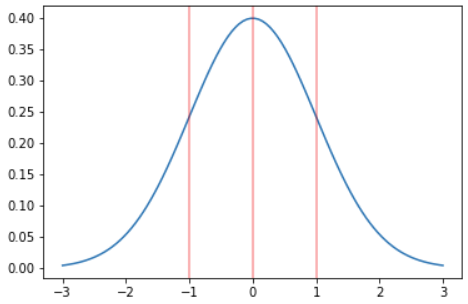
\includegraphics[width=0.75\textwidth]{sd_3.png}
    \caption[short]{$\mu$ +/- [1]$\sigma$ \\with 2,000 iterations.}
    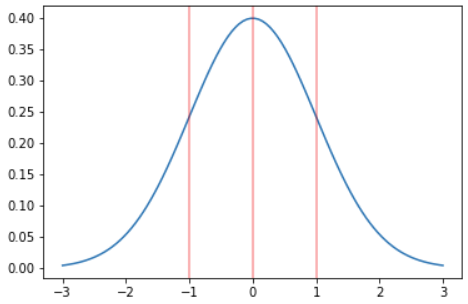
\includegraphics[width=0.75\textwidth]{sd_3.png}
    \caption[short]{$\mu$ +/- [1,2]$\sigma$ \\with 2,000 iterations.}
    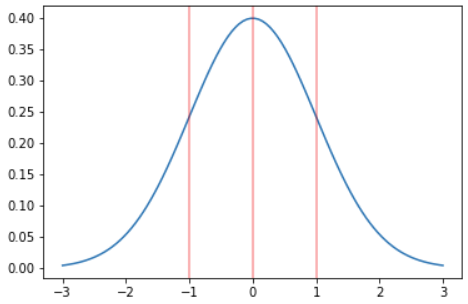
\includegraphics[width=0.75\textwidth]{sd_3.png}
    \caption[short]{$\mu$ +/- [1,2,3]$\sigma$ \\with 2,000 iterations.}
\end{subfigure}
\end{figure}


\newpage
If we were implementing a difference of means t-test, then we could simply apply the formula below to get the appropriate sample size.
\[n = 2 \Bigg(\frac{Z_{1-(\alpha/2)}+Z_{1-\beta}}{ES}\Bigg)^2 \text{  where  } ES = \frac{|\mu_1-\mu_2|}{\sigma}\]

Here, $\alpha$ is the probability of a Type I error (false rejection of the NULL hypothesus, i.e. a false positive) and $\beta$ is the probability of a Type II error (i.e. a false negative). Observe how if we want to make our test more rigorous and reduce the false positive rate, the the left side of the numerator increase and the resulting recommended sample size - $n$, also increases. Similarly, if we want to reduce the probability for failing to detect the difference across groups, then we will need to increase the right-hand side of the numerator - also increasing the recommended sample size.

\newpage
\[ y = \beta_0 + \mathlarger{\mathlarger{\mathlarger{\mathlarger{\mathlarger{\mathlarger{\epsilon}}}}}} \]
\[ y = \beta_0 + X_1\beta_1 + \mathlarger{\mathlarger{\mathlarger{\epsilon}}}\]
\[ y = \beta_0 + X_1\beta_1 + X_2\beta_2 + \mathlarger{\mathlarger{\epsilon}}\]
\[ y = \beta_0 + X_1\beta_1 + X_2\beta_2 + X_3\beta_3 +\mathlarger{\epsilon}\]
\[ y = \beta_0 + ... + \beta_nX_n + \epsilon \text{\phantom{aa} where \phantom{aa}} \hat{\epsilon} = y - \hat{y}\]

\newpage
\[\text{In our ongoing effort to predict the amount spent on an individual order, let's try the following...}\]
\[ y = \beta_0 + \beta_1X_1 + \beta_2X_2 + \beta_3X_3 + \beta_4X_4 +\mathlarger{\epsilon}\]
\[\text{where } X_1 \text{ is whether the customer was assigned the treatment...}\]
\[X_2 \text{ is the customer's mean order amount prior to treatment...}\]
\[X_3 \text{ is the retailer's mean order amount prior to treatment...}\]
\[X_4 \text{ is the mean order amount for that day of the week prior to treatment...}\]
\[\epsilon \text{ is unaccounted for variation in $y$, and } \hat{\epsilon} = y - \hat{y}\]



\newpage

\begin{landscape}
\begin{center}
\Large{Required Sample Size Estimates Taken Via Analysis of Residual Variance}
\end{center}
\begin{table}[h]
\small\addtolength{\tabcolsep}{-1pt}
\begin{tabular}{c|cccccccccccccccc}
                                                                                         & \textbf{I}                                               & \textbf{II}                                              & \textbf{III}                                             & \textbf{IV}                                               & \textbf{V}                                              & \textbf{VI}                                              & \textbf{VII}                                            & \textbf{VIII}                                          & \textbf{IX}                                              & \textbf{X}                                               & \textbf{XI}                                              & \textbf{XII}                                           & \textbf{XIII}                                           & \textbf{XIV}                                            & \textbf{XV}                                             & \textbf{XVI}                                             \\ \hline
\textbf{\begin{tabular}[c]{@{}c@{}}\small{Mean Diff.} \\ \small{in Estimated} \\ \small{Power (Std.)}\end{tabular}} & \begin{tabular}[c]{@{}c@{}}\small{-0.723}\\ \smaller{(0.011)}\end{tabular} & \begin{tabular}[c]{@{}c@{}}\small{-0.683}\\ \smaller{(0.014)}\end{tabular} & \begin{tabular}[c]{@{}c@{}}\small{-0.541}\\ \smaller{(0.018)}\end{tabular} & \begin{tabular}[c]{@{}c@{}}\small{-0.387}\\ \smaller{(-0.022)}\end{tabular} & \begin{tabular}[c]{@{}c@{}}\small{0.198}\\ \smaller{(0.002)}\end{tabular} & \begin{tabular}[c]{@{}c@{}}\small{0.199}\\ \smaller{($<$0.01)}\end{tabular} & \begin{tabular}[c]{@{}c@{}}\small{0.199}\\ \smaller{($<$0.01})\end{tabular} & \begin{tabular}[c]{@{}c@{}}\small{0.143}\\ \smaller{(0.01)}\end{tabular} & \begin{tabular}[c]{@{}c@{}}\small{0.199}\\ \smaller{($<$0.01)}\end{tabular} & \begin{tabular}[c]{@{}c@{}}\small{0.199}\\ \smaller{($<$0.01)}\end{tabular} & \begin{tabular}[c]{@{}c@{}}\small{0.199}\\ \smaller{($<$0.01)}\end{tabular} & \begin{tabular}[c]{@{}c@{}}\small{0.105}\\ \smaller{(0.01)}\end{tabular} & \begin{tabular}[c]{@{}c@{}}\small{0.189}\\ \smaller{($<$0.01)}\end{tabular} & \begin{tabular}[c]{@{}c@{}}\small{0.192}\\ \smaller{($<$0.01)}\end{tabular} & \begin{tabular}[c]{@{}c@{}}\small{0.185}\\ \small{($<$0.01)}\end{tabular} & \begin{tabular}[c]{@{}c@{}}\small{-0.124}\\ \smaller{(0.023)}\end{tabular} \\ \hline
\textbf{\begin{tabular}[c]{@{}c@{}}\small{Mean} \\  \small{Estimated} \\ \small{Sample} \\ \small{Size (Std.)}\end{tabular}}    & 
\begin{tabular}[c]{@{}c@{}}\small{31} \\ \small{(0.43)}\end{tabular} &          
\begin{tabular}[c]{@{}c@{}}\small{123} \\ \small{(1.2)}\end{tabular} &       
\begin{tabular}[c]{@{}c@{}}\small{689} \\ \small{(5.7)}\end{tabular} &  
\begin{tabular}[c]{@{}c@{}}\small{3,836} \\ \small{(36.2)}\end{tabular} &    
\begin{tabular}[c]{@{}c@{}}\small{3,836} \\ \small{(19.2)}\end{tabular} &  
\begin{tabular}[c]{@{}c@{}}\small{14,017} \\ \small{(68.0)}\end{tabular} &
\begin{tabular}[c]{@{}c@{}}\small{83,711} \\ \small{(435.7)}\end{tabular} &
\begin{tabular}[c]{@{}c@{}}\small{460,231} \\ \small{(2,183.2)}\end{tabular} &
\begin{tabular}[c]{@{}c@{}}\small{3,847} \\ \small{(23.6)}\end{tabular} &
\begin{tabular}[c]{@{}c@{}}\small{14,055} \\ \small{(77.07)}\end{tabular} &
\begin{tabular}[c]{@{}c@{}}\small{83,954} \\ \small{(512.8)}\end{tabular} &
\begin{tabular}[c]{@{}c@{}}\small{461,663} \\ \small{(2370.2)}\end{tabular} &
\begin{tabular}[c]{@{}c@{}}\small{4,093} \\ \small{(25.6)}\end{tabular} &
\begin{tabular}[c]{@{}c@{}}\small{14,904} \\ \small{(84.3)}\end{tabular} &
\begin{tabular}[c]{@{}c@{}}\small{88,932} \\ \small{(504.0)}\end{tabular} &
\begin{tabular}[c]{@{}c@{}}\small{491,528} \\ \small{(2,927.6)}\end{tabular}               
\\ \hline
\textbf{\begin{tabular}[c]{@{}c@{}}Mean \\ Adjusted $R^2$ \end{tabular}}   & 0.99                                                     & 0.96                                                     & 0.94                                                     & 0.93                                                      & 0.49                                                    & 0.41                                                     & 0.38                                                    & 0.38                                                   & 0.36                                                     & 0.36                                                     & 0.36                                                     & 0.36                                                   & 0.004                                                   & 0.001                                                   & 0.0                                                     & 0.0                                                      \\ \hline
\textbf{\begin{tabular}[c]{@{}c@{}}Verification \\ Simulations\end{tabular}}             & 500                                                      & 500                                                      & 500                                                      & 500                                                       & 500                                                     & 500                                                      & 500                                                     & 500                                                    & 500                                                      & 500                                                      & 500                                                      & 500                                                    & 500                                                     & 500                                                     & 500                                                     & 500                                                     
\end{tabular}
\end{table}
\begin{center}
Simulations were conducted on dual Intel Xeon CPU E5-2670 processors.
\end{center}
\end{landscape}

\newpage
\[ \text{Let } Pr(p<0.05) = 1-e^{-\lambda x} \text{ where $x$ is the number of observations}\] 
\[\text{sampled and the alternative hypothesis is true.} \]



\end{document}